\chapter{Supplementary Material for Chapter~\ref{sec:06_lgae}}
\label{app:06}

\section{Model details}
\label{app:06_lgae_hyperparams}

\subsection{LGAE}

For both the encoder and decoder, we choose $N_\mathrm{MP}^\mathrm{E} = N_\mathrm{MP}^\mathrm{D} = 4$ LMP layers.
The multiplicity per node in each LMP layer has been optimized to be
\begin{equation}
    \left\{ \parenthesis{\tau_{(m, n)}^{(t)}}^\mathrm{E} \right\}_{t=1}^{4} = (3,3,4,4)
\end{equation}
for the encoder and
\begin{equation}
    \left\{ \parenthesis{\tau_{(m, n)}^{(t)}}^\mathrm{D} \right\}_{t=1}^{4} = (4,4,3,3)
\end{equation}
for the decoder, the components in the vector on the right-hand side are the multiplicity in each of the four LMP layers per network, and the multiplicity per layer is the same for all representations.
After each CG decomposition, we truncate irreps of dimensions higher than $(1/2, 1/2)$ for tractable computations, i.e., after each LMP operation we are left with only scalar and vector representations per node.
Empirically, we did not find such a truncation to affect the performance of the model.
This means that the LMP layers in the LGAE are similar in practice to those of LorentzNet, which uses only scalar and vector representations throughout, but are more general as higher dimensional representations are involved in the intermediate steps before truncation.

The differentiable mapping $f(d_{ij})$ in Eq.~\ref{eq:06_lgae_msg} is chosen to be the Lorentzian bell function as in Ref.~\cite{bogatskiy2020lorentz}.
For all models, the latent space contains only $\tau_{(0,0)} = 1$ complex Lorentz scalar, as we found increasing the number of scalars beyond one did not improve the performance in either reconstruction or anomaly detection.
Empirically, the reconstruction performance increased with more latent vectors, as one might expect, while anomaly detection performance generally worsened from adding more than two latent vectors.

\subsection{GNNAE}
The GNNAE is constructed from fully-connected MPNNs.
The update rule in the $(t+1)$-th MPNN layer is based on MPGAN's (Section~\ref{sec:04_mpgan}), and given by
\begin{align}
    m_i^{(t)}   & = \sum_{j=1}^n f_e^{(t)}\left(
    x_i^{(t)} \oplus x_j^{(t)} \oplus d\left(x_i^{(t)}, x_j^{(t)}\right)
    \right), \label{eq:06_lgae_gnnae-m}                  \\
    x_i^{(t+1)} & = f_n^{(t)} \left(
    x_i^{(t)} \oplus m_i^{(t)}
    \right), \label{eq:06_lgae_gnnae-x}
\end{align}
where $x_i^{(t)}$ is the node embedding of node $i$ at $t$-th iteration,
$d$ is any distance function (Euclidean norm in our case),
$m_i^{(t)}$ is the message for updating node embedding in node $i$,
$f_e^{(t+1)}$ and $f_n^{(t+1)}$ are any learnable mapping at the current MP layer.
A diagram for an MPNN layer is shown in Figure~\ref{fig:06_lgae_gnn-message-passing}.
The overall architecture is similar to that in Figure~\ref{fig:06_lgae_architecture-full}, with the LMP replaced by the MPNN.
The code for the GNNAE model can be found in the Ref.~\cite{GNNAE_code}.

\begin{figure}[htpb]
    \centering
    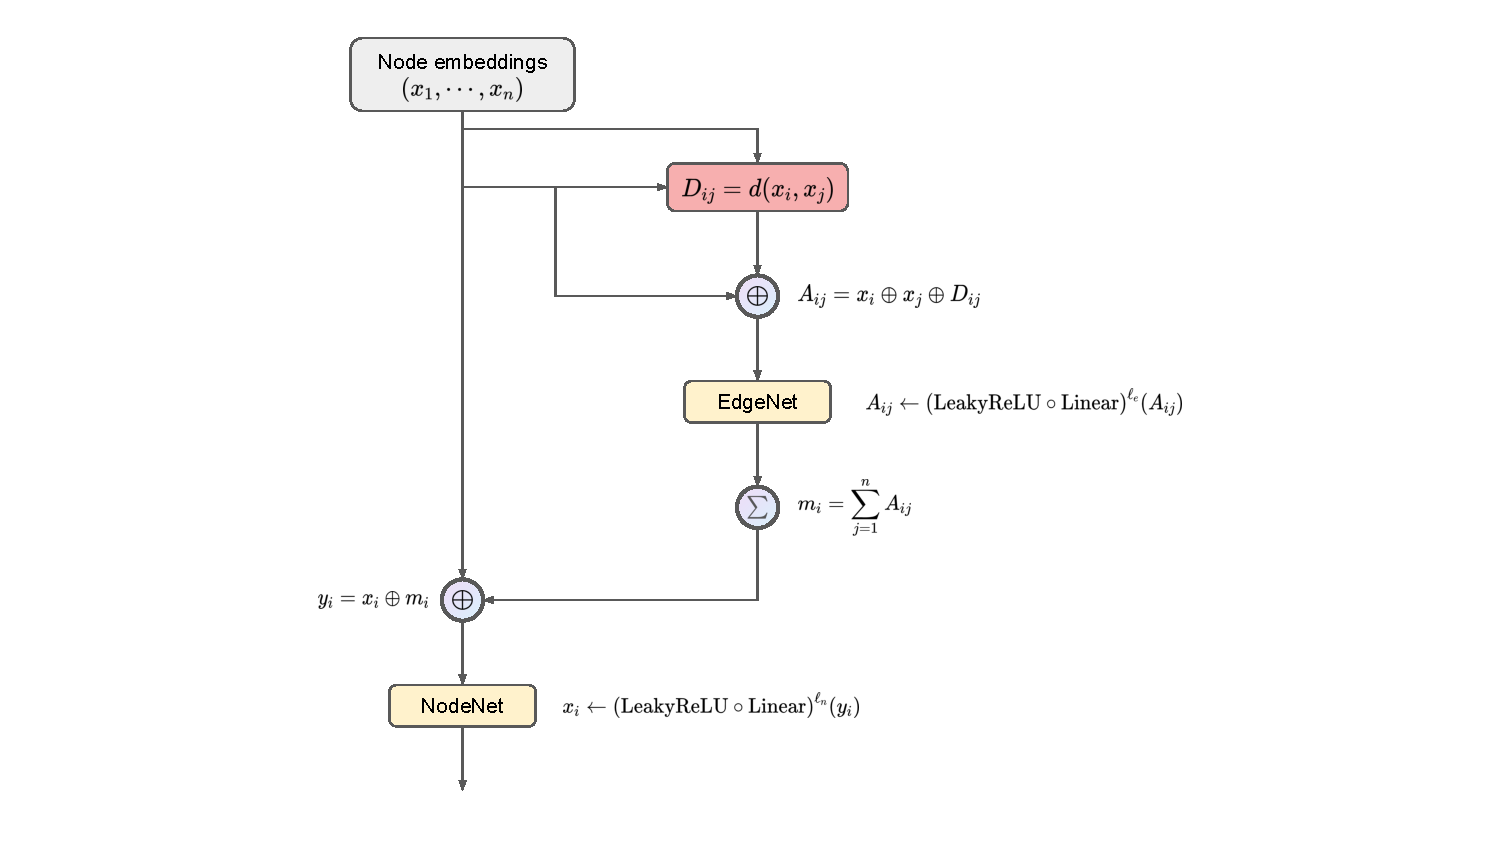
\includegraphics[scale=0.55]{figures/06-ML4Jets/lgae/architectures/GNNAE-MPNN.pdf}
    \caption{An MPNN layer in the GNNAE. Here, $\mathrm{EdgeNet}$ and $\mathrm{NodeNet}$ are feed-forward neural networks.}
    \label{fig:06_lgae_gnn-message-passing}
\end{figure}

For both the encoder and decoder, there are $3$ MPNN layers.
The learnable functions in each layer are optimized to be
\begin{equation}
    \begin{split}
        f_n^{(1)} &= (
        \mathrm{LeakyReLU}_{0.2}
        \circ
        \mathrm{Linear}_{30\to 15}) \\
        &\quad \circ
        (\mathrm{LeakyReLU}_{0.2}
        \circ
        \mathrm{Linear}_{60\to 30}) \\
        f_e^{(1)} &=
        (\mathrm{LeakyReLU}_{0.2}
        \circ
        \mathrm{Linear}_{40\to 30}), \\
        &\quad \circ
        (\mathrm{LeakyReLU}_{0.2}
        \circ
        \mathrm{Linear}_{50\to 40}) \\
        &\quad \circ
        (\mathrm{LeakyReLU}_{0.2}
        \circ
        \mathrm{Linear}_{61\to 50}),
    \end{split}
\end{equation}
\begin{equation}
    \begin{split}
        f_n^{(2)} &= (
        \mathrm{LeakyReLU}_{0.2}
        \circ
        \mathrm{Linear}_{15\to 8}) \\
        &\quad \circ
        (\mathrm{LeakyReLU}_{0.2}
        \circ
        \mathrm{Linear}_{45\to 15}) \\
        f_e^{(2)} &=
        (\mathrm{LeakyReLU}_{0.2}
        \circ
        \mathrm{Linear}_{31\to 30}), \\
        &\quad \circ
        (\mathrm{LeakyReLU}_{0.2}
        \circ
        \mathrm{Linear}_{30\to 30}) \\
        &\quad \circ
        (\mathrm{LeakyReLU}_{0.2}
        \circ
        \mathrm{Linear}_{30\to 30}),
    \end{split}
\end{equation}
\begin{equation}
    \begin{split}
        f_n^{(3)} &= (
        \mathrm{LeakyReLU}_{0.2}
        \circ
        \mathrm{Linear}_{8 \to \delta}) \\
        &\quad \circ
        (\mathrm{LeakyReLU}_{0.2}
        \circ
        \mathrm{Linear}_{38\to 8}) \\
        f_e^{(3)} &=
        (\mathrm{LeakyReLU}_{0.2}
        \circ
        \mathrm{Linear}_{20\to 30}), \\
        &\quad \circ
        (\mathrm{LeakyReLU}_{0.2}
        \circ
        \mathrm{Linear}_{16\to 20}) \\
        &\quad \circ
        (\mathrm{LeakyReLU}_{0.2}
        \circ
        \mathrm{Linear}_{17\to 16}),
    \end{split}
\end{equation}
where $\mathrm{LeakyReLU}_{0.2}(x) = \max(0.2 x, x)$ is the LeakyReLU function.

Depending on the aggregation layer, the value of $\delta$ in $f_n^{(3)}$ and the final aggregation layer is different.
For GNNAE-JL encoders, $\delta = N \times \dim(L)$, where $L$ is the latent space, and $N$ is the number of nodes in the graph.
Then, mean aggregation is done across the graph.
For GNNAE-PL encoders, $\delta = d$, where $d$ is the node dimension in the latent space.
In the GNNAE-JL decoder, the input layer is a linear layer that recovers the particle cloud structure similar to that in the LGAE.

\subsection{CNNAE}
The encoder is composed of two convolutional layers with kernel size $(3, 3)$, stride size $(2, 2)$, ``same" padding, and $128$ output channels, each followed by a ReLU activation function. 
The aggregation layer into the latent space is a fully-connected linear layer. 
The decoder is composed of transposed convolution layers (also known as deconvolutional layers) with the same settings as the encoder. 
A softmax function is applied at the end so that the sum of all pixel values in an image is $1$, as a property of the jet image representation.
A 55-dimensional latent space  is chosen so that the compression rate is $55/90 \approx 60\%$ for even comparisons with the LGAE and GNNAE models.



\section{Training details}
\label{app:06_lgae_training}
We use the Chamfer loss function~\cite{10.5555/1622943.1622971,Fan_2017_CVPR,Zhang2020FSPool} for the LGAE-Min-Max and GNNAE-JL models, and  MSE for LGAE-Mix and GNNAE-PL.
We tested the Hungarian loss~\cite{hungarian,2020SciPy-NMeth} and differentiable energy mover's distance (EMD)~\cite{Komiske:2019fks}, calculated using the \jetnet library~\cite{jetnetlibrary}, as well but found the Chamfer and MSE losses more performant.

The graph-based models are optimized using the Adam optimizer~\cite{kigma2015adam}
implemented in \textsc{PyTorch}~\cite{pytorch}
with a learning rate $\gamma = 10^{-3}$, coefficients $(\beta_1, \beta_2) = (0.9, 0.999)$, and weight decay $\lambda = 0$.
The CNNAE is optimized using the same optimizer implemented in TensorFlow~\cite{tensorflow2015-whitepaper}. 
They are all trained on single NVIDIA RTX 2080 Ti GPUs each for a maximum of 20000 epochs using early stopping with the patience of 200 epochs.
The total training time for LGAE models is typically 35 hours, and at most 100 hours, while GNNAE-PL and GNNAE-JL train for 50 and 120 hours on average, respectively.
By contrast, the CNNAE model, due to its simplicity, can typically converge within 3 hours.



\section{Equivariance tests}
\label{app:06_lgae_equivariancetests}

We test the covariance of the LGAE models to Lorentz transformations and find they are indeed equivariant up to numerical errors.
Reference~\cite{bogatskiy2020lorentz} points out that equivariance to boosts in particular is sensitive to numerical precision, so we use double precision (64-bit) throughout the model. 
In addition, we scale down the data by a factor of 1,000 (i.e. working in the units of PeV) for better numerical precision at high boosts.

For a given transformation $\Lambda \in \mathrm{SO}^+(3,1)$ we compare $\Lambda \cdot \mathrm{LGAE}(p)$ and $ \mathrm{LGAE}(\Lambda \cdot p)$ are compared, where $p$ is the particle-level 4-momentum. 
The relative deviation is defined as
\begin{equation} \label{eq:06_lgae_delta-p}
    \delta_p(\Lambda) = \left|\frac{
        \mathrm{mean}(\mathrm{LGAE}(\Lambda \cdot p)) -
        \mathrm{mean}(\Lambda \cdot \mathrm{LGAE}(p))
    }{\mathrm{mean}(\Lambda \cdot \mathrm{LGAE}(p))}\right|
\end{equation}
Figure~\ref{fig:06_lgae_equivariance} shows the mean relative deviation, averaged over each particle in each jet, over $3000$ jets from our test dataset from boosts along and rotations around the $z$-axis.
We find the relative deviation from boosts to be within $\order{10^{-3}}$ in the interval $\gamma \in [0, \cosh(10)]$ (equivalent to $\beta \in [0, 1 - 4\times10^{-9}$]) and from rotations to be $<10^{12}$. 

\begin{figure}[ht]
    \centering
    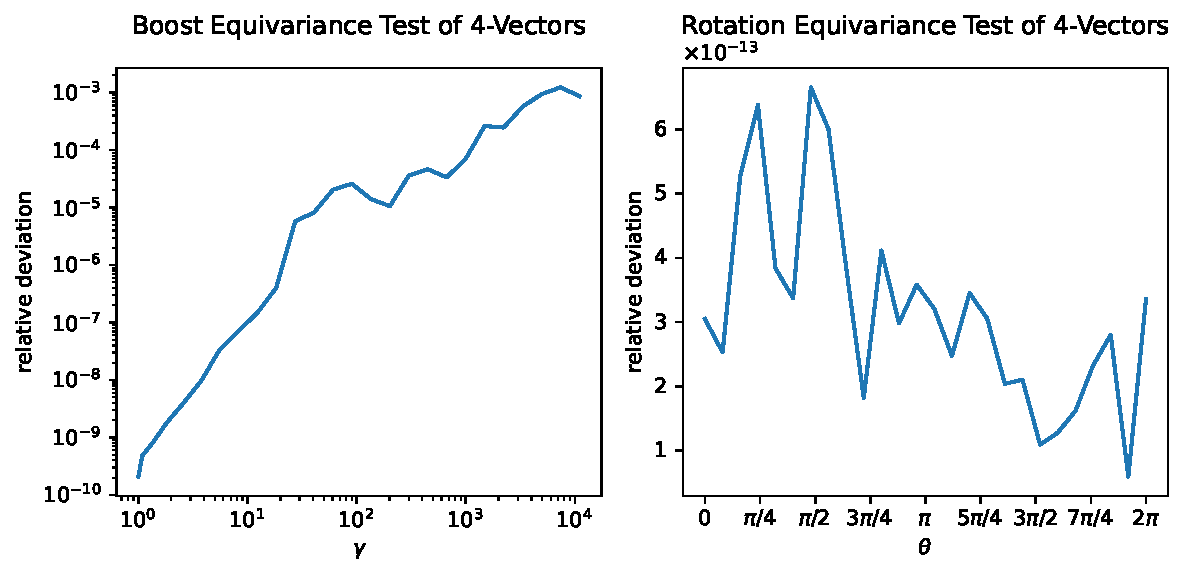
\includegraphics[width=\linewidth]{figures/06-ML4Jets/lgae/covariance/equivariance-p4.pdf}
    \caption{The relative deviations, as defined in Eq.~\ref{eq:06_lgae_delta-p}, of the output 4-momenta $p^\mu$ to boosts along the $z$-axis (left) and rotations around the $z$-axis (right).}
    \label{fig:06_lgae_equivariance}
\end{figure}